% ============================================================
%  孟凡腾 — 个人简历（Curriculum Vitae，中文版）
%  编译方式：xelatex cv_CN.tex
% ============================================================
\documentclass[11pt,a4paper]{ctexart}

% ---- Packages ----
\usepackage[margin=0.85in]{geometry}
\usepackage{enumitem}
\usepackage{titlesec}
\usepackage{xcolor}
\usepackage{tabularx}
\usepackage{graphicx}              % 证件照

% ---- Colors ----
\definecolor{sectioncolor}{RGB}{0,51,145}
\definecolor{accent}{RGB}{100,80,155}
\definecolor{graytext}{RGB}{100,100,100}
\definecolor{linkcolor}{RGB}{60,80,160}

\usepackage[colorlinks=true,
  linkcolor=linkcolor,
  urlcolor=linkcolor,
  pdftitle={孟凡腾 -- 简历},
  pdfauthor={孟凡腾}]{hyperref}

% ---- Section formatting ----
\titleformat{\section}
  {\sffamily\bfseries\large\color{sectioncolor}}
  {\thesection}{1em}{}[\vspace{-3pt}\textcolor{sectioncolor}{\rule{\textwidth}{0.6pt}}\vspace{-6pt}]
\titlespacing*{\section}{0pt}{12pt}{8pt}

% ---- Custom environments ----
\newenvironment{entrylist}
  {\begin{itemize}[leftmargin=*,nosep,itemsep=2pt]}
  {\end{itemize}}

\newlength{\datelabelwidth}
\newcommand{\cvitem}[3]{%
  \setlength{\datelabelwidth}{2.8cm}%
  \noindent%
  \parbox[t]{\datelabelwidth}{\raggedleft\footnotesize\sffamily\color{graytext}#1}%
  \hspace{0.6cm}%
  \parbox[t]{\dimexpr\textwidth-\datelabelwidth-0.6cm\relax}{%
    \textbf{#2}\par\small#3\par}%
  \vspace{2.5mm}\par%
}

% ---- Header ----
\newcommand{\makecvheader}{%
  \noindent
  \begin{minipage}[t]{3.7cm}
    \vspace{0.1em}
    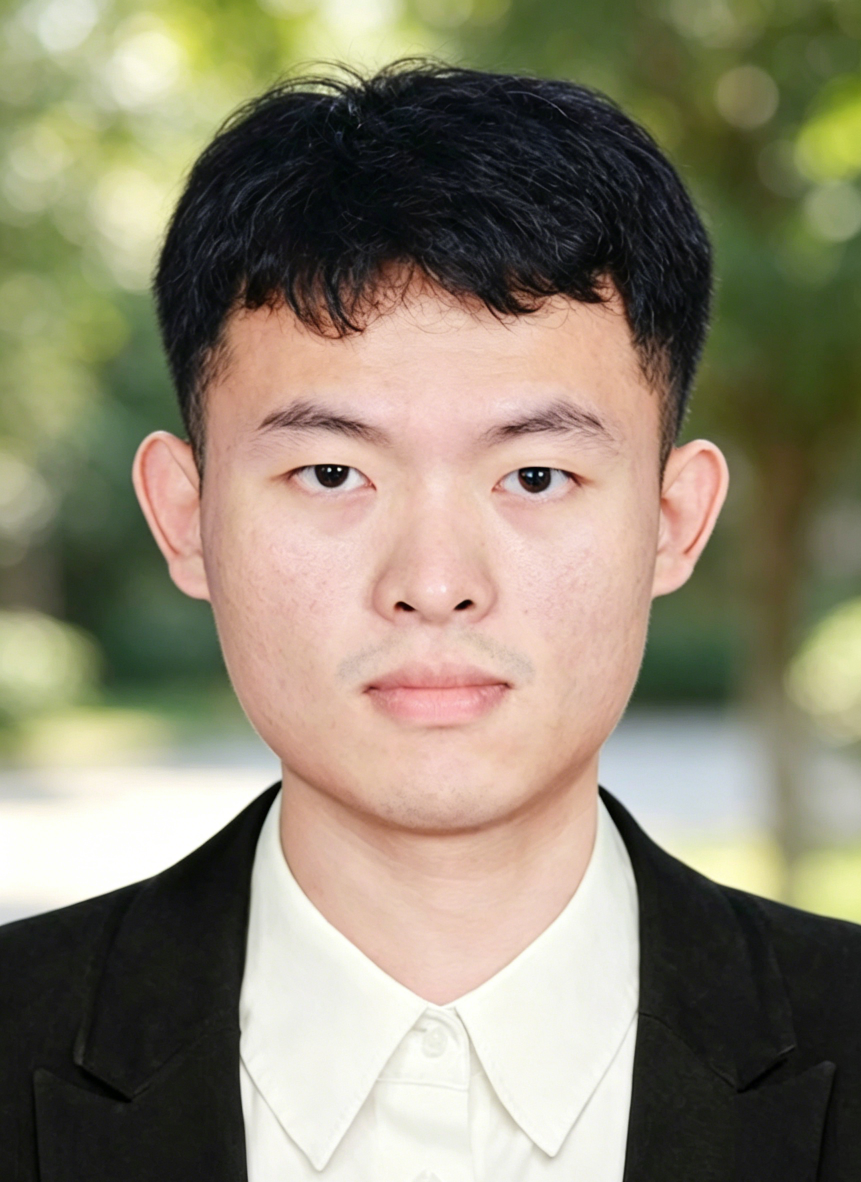
\includegraphics[height=3.65cm,keepaspectratio,clip]{../images/photo-202601-square.png}%
  \end{minipage}\hspace{1.1em}%
  \begin{minipage}[t]{0.60\textwidth}
    \vspace{0.7em}
    {\fontsize{22}{26}\selectfont\sffamily\bfseries 孟凡腾}\par
    \vspace{1pt}\color{graytext}\large 安全科学与工程专业博士生\par
    \vspace{6pt}\small
    \href{mailto:ftmeng@bjtu.edu.cn}{ftmeng@bjtu.edu.cn}\,
    $\cdot$\,
    \href{https://ft115.github.io}{ft115.github.io}\,
    $\cdot$\,
    \href{https://scholar.google.com.hk/citations?user=Yq5wnc8AAAAJ}{Google Scholar}\par
    \vspace{3pt}\footnotesize\color{graytext}北京交通大学 · 先进轨道交通自主运行全国重点实验室\\[1pt]
    \footnotesize\color{graytext}北京交通大学 · 交通运输学院（智能系），北京，中国
  \end{minipage}
  \par\vspace{3pt}
  \noindent\textcolor{black}{\rule{\textwidth}{0.4pt}}\vspace{5pt}
}

\begin{document}
\widowpenalty=10000
\clubpenalty=10000
\brokenpenalty=10000
\displaywidowpenalty=10000

\makecvheader

% ============================================================
\section{教育经历}

\cvitem{2023 -- 至今}
  {博士，安全科学与工程}
  {北京交通大学，先进轨道交通自主运行全国重点实验室\\
   交通运输学院（智能系）\\
   导师：秦勇 教授\\
   自 2023 年起硕博连读。}

\cvitem{2022 -- 2023}
  {硕士，交通运输规划与管理}
  {北京交通大学}

\cvitem{2018 -- 2022}
  {本科，交通运输}
  {石家庄铁道大学}

% ============================================================
\section{研究方向}

\noindent
无人机智能巡检；轨道交通机器视觉与深度学习；
边缘计算；三维重建与点云分析。

% ============================================================
\section{科研项目}

\begin{enumerate}[leftmargin=1.9em,itemsep=3pt,label=\arabic*.]
  \item \textbf{自主化轨道交通系统安全保障技术与示范验证}（2022--2026）· 国家重点研发计划 · 核心参与
  \item \textbf{基于无人机遥感图像的高铁沿线环境未知风险识别技术研究}（2024--2026）· 中央高校基本科研专项 · \textbf{主持}
  \item \textbf{高铁基础设施无人机巡检技术深化研究及应用}（2022--2024）· 国铁集团“重大项目” · 核心参与
  \item \textbf{京沪高铁基础设施无人机智能巡检系统建设}（2023--2024）· 京沪高铁“重大项目” · 核心参与
  \item \textbf{铁路钢桥涂装自动化检修设备及关键技术研究}（2024--2027）· 京沪高铁“重大项目” · 核心参与
  \item \textbf{青藏铁路桥梁关键区域缺陷及落石异物的自主无人机智能巡检技术应用}（2026--2027）· 青藏铁路“智慧天路”重大项目 · 核心参与
\end{enumerate}

% ============================================================
\section{代表性论文}

\noindent\textit{* 通讯作者；$^\#$ 共同第一作者。}

\begin{enumerate}[leftmargin=*,nosep,itemsep=3pt]
  \item \textbf{Meng, F.}, Qin, Y.$^*$, Wu, Y.$^*$, et al.\
    ``SRLF: Sparse Representation Learning Framework for Railroad Surrounding Potential Risk Perception Using UAV Imagery.''
    \textit{IEEE Trans.\ Intell.\ Transp.\ Syst.}, 2025.\\
    {\small\color{graytext}（中科院 1 区 TOP；5 年 IF 10.403）}

  \item \textbf{Meng, F.}, Qin, Y.$^*$, Wu, Y.$^*$, Shao, C., Yang, H., Jia, L.\
    ``Automatic Risk Level Evaluation System for Potential Environmental Hazards along High-speed Railroad Using UAV Aerial Photograph.''
    \textit{Expert Syst.\ Appl.}, 2025.\\
    {\small\color{graytext}（Expert Systems with Applications，中科院 1 区 TOP；5 年 IF 8.995）}

  \item \textbf{Meng, F.}, Qin, Y.$^*$, Wu, Y.$^*$, Shao, C., Jia, L.\
    ``A Subtle Defect Recognition Method for Catenary Fastener in High-speed Railroad Using Destruction and Reconstruction Learning.''
    \textit{Adv.\ Eng.\ Inform.}, 2024.\\
    {\small\color{graytext}（Advanced Engineering Informatics，中科院 1 区 TOP；5 年 IF 11.204）}

  \item Wu, Y.$^\#$, \textbf{Meng, F.}$^\#$, Qin, Y.$^*$, Qian, Y.$^*$, Xu, F., Jia, L.\
    ``UAV Imagery Based Potential Safety Hazard Evaluation for High-speed Railroad Using Real-time Instance Segmentation.''
    \textit{Adv.\ Eng.\ Inform.}, 2023.\\
    {\small\color{graytext}（Advanced Engineering Informatics，中科院 1 区 TOP；5 年 IF 11.204）}

  \item Wu, Y.$^\#$, \textbf{Meng, F.}$^\#$, Qin, Y.$^*$, Qian, Y.$^*$, Liu, Z., Zhao, W.\
    ``Automated Anomaly Detection of Catenary Split Pins Using Unsupervised Learning.''
    \textit{Autom.\ Constr.}, 2024.\\
    {\small\color{graytext}（Automation in Construction，中科院 1 区 TOP；5 年 IF 13.598）}

  \item \textbf{孟凡腾}，秦勇$^{*}$，崔京，等.\
    ``铁路外部环境无人机图像未知风险检测方法.''
    \textit{航空学报（Acta Aeronautica et Astronautica Sinica）}, 2025.\\
    {\small\color{graytext}（《航空学报》：中文航空领域权威期刊，中国科技期刊卓越行动计划 T1，EI 收录）}

  \item 秦勇$^{*}$，\textbf{孟凡腾}$^{\#}$，张紫城，等.\
    ``轨道交通基础设施自主无人机智能巡检体系框架及其技术发展综述.''
    \textit{北京交通大学学报}, 2025.\\
    {\small\color{graytext}（《北京交通大学学报》：北大核心、CSCD 收录）}
\end{enumerate}

% ============================================================
\section{代表性工程实践}

\begin{enumerate}[leftmargin=*,nosep,itemsep=4pt]

  \item \textbf{高速铁路全自动无人机智能巡检系统}
  \begin{itemize}[leftmargin=*,nosep]
    \item 国内外首套高速铁路无人机自主智能巡检系统，规模应用近百公里。
    \item 国家重点研发计划核心研究人员；设计 3 项原创视觉算法（召回率 \textgreater{}96\%）。
    \item 部署 6 架巡检无人机 + 4 套自动化机巢；较人工巡检效率提升 10 倍以上。
  \end{itemize}

  \item \textbf{青藏铁路桥梁与落石灾害无人机智能巡检}
  \begin{itemize}[leftmargin=*,nosep]
    \item 平均海拔 3000+ 米自主飞行巡检。
    \item 全栈技术研发：自主飞行控制、摄影测量三维重建、点云分割。
    \item 多期点云配准与落石形变检测，服务高原铁路运营安全。
  \end{itemize}

  \item \textbf{铁路钢桁梁桥无人机全覆盖巡检与涂层缺陷评估}
  \begin{itemize}[leftmargin=*,nosep]
    \item GNSS 拒止下大跨度铁路钢桥飞行巡检。
    \item 设计覆盖桥顶、桥侧及复杂桥底区域的避障巡检航线。
    \item 端到端流程：涂层缺陷识别 $\to$ 量化分级 $\to$ 缺陷空间溯源。
  \end{itemize}

\end{enumerate}

% ============================================================
\section{专利}

\noindent\textbf{已授权专利}

\begin{enumerate}[leftmargin=*,nosep,itemsep=2pt]
  \item Autonomous UAV Based Intelligent Inspection System for Equipment, Facilities, and the Environment along Railway Lines and Method Thereof.（美国发明专利）
  \item 基于无人机图像的铁路环境隐患识别与风险等级评估方法
  \item 用于卫星拒止下交通设施巡检的无人机航线生成方法
  \item 跨模态自适应匹配的激光雷达与相机的在线外参标定方法及系统
\end{enumerate}

\noindent\textbf{已公开专利申请}

\begin{enumerate}[leftmargin=*,nosep,itemsep=2pt]
  \item 用于无人机遥感图像的铁路沿线环境未知风险识别方法
  \item 一种用于铁路接触网的开口销缺陷精细化识别方法
  \item 铁路钢桁架桥涂层锈蚀检测评估方法及系统
\end{enumerate}

% ============================================================
\section{荣誉与获奖}

\begin{itemize}[leftmargin=*,nosep,itemsep=2pt]
  \item[2024] 世界互联网大会领先科技奖优秀成果——“轨道交通全自主无人机智能巡检技术及应用”
  \item[2024] 第十四届“挑战杯”中国大学生创业计划竞赛“一带一路”国际邀请赛 银奖
  \item[2024] “青创北京”首都大学生挑战杯创业计划竞赛 银奖
  \item[2022] 北京交通大学暑期深度学习训练营 二等奖（第二名）
  \item[2021] 中国交通优秀学子 一等奖（首奖）
  \item[2021] 第七届全国大学生工程训练综合能力竞赛 省级一等奖
  \item[2021] 省级三好学生
  \item[2020] 第十二届全国大学生数学竞赛 省级一等奖
  \item[2020] 第七届全国大学生物理竞赛 省级一等奖
\end{itemize}

% ============================================================
\section{学术服务}

\noindent\textbf{期刊审稿人}\quad
\textit{IEEE Trans.\ Intell.\ Transp.\ Syst.} (T-ITS),
\textit{Adv.\ Eng.\ Inform.} (AEI),
\textit{Expert Syst.\ Appl.} (ESWA)

% ============================================================
\section{专业技能}

\noindent
\textbf{编程语言与框架：}\ \ Python, C++, Matlab
\quad
\textbf{深度学习：}\ \ PyTorch
\quad
\textbf{系统平台：}\ \ Linux, ROS
\quad
\textbf{视觉处理：}\ \ OpenCV
\quad
\textbf{硬件/机载：}\ \ DJI-PSDK

\end{document}
